\chap{Uvod}
%\sect{Matematične osnove}
%\newpage
%\sect{Notacija}
%\begin{itemize}
%	\item[Množice:] Označimo z velikimi tiskanimi črkami. Podamo jih lahko na naslednje načine\\
%	$ A = \{ a_1, a_1, a_3, \ldots \} $ - naštevanje elementov\\
%	$ B = \{ n | \ \mbox{pravilo za n} \} \ $ - opis elementov
%\end{itemize}

%?appendix this:
%\chapter{Slovar}
%?zihr obstaja neki za to, sicer naredi definitions okolje
%\begin{items}
%\item Razred - razred je množica elementov, ki ga lahko podamo z naštevanjem elementov ali z opisom lastnosti (opisni ali konceptualni razredi)
%\end{items}

\sect{Osnove dokazovanja}
\subsect{Dokaz s konstrukcijo}
Dokaz obstoja nekega matematičnega objekta je to, da nam ga uspe sestaviti.

\begin{primeri}
\item Za vsak $n>4$, obstaja dvojiško drevo, ki ima natanko $3$ liste.\\
	Primer za $n=5$:
	\br
	\hspace*{1cm}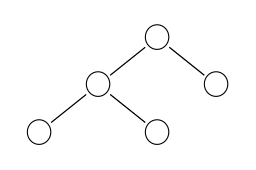
\begin{tikzpicture}[level distance=6mm, inner sep=-0.3mm]
		\node (root) {$\bigcirc$}
		child { node (a) {$\bigcirc$} 
			child { node (b) {$\bigcirc$} }
			child { node (c) {$\bigcirc$} }
		}
		child { node (d) {$\bigcirc$} };
	\end{tikzpicture}
	\br
	Primer za $n>5$, pri čemer je "$...$", poljubno vejitev samo v levo:
	\br
	\hspace*{1cm}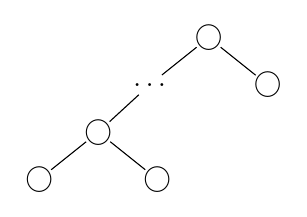
\begin{tikzpicture}[level distance=6mm, inner sep=-0.3mm]
		\node (root) {$\bigcirc$}
		child { node (a) [inner sep=1mm] {$\dots$} {
			child { node (b) [left=0.5cm] {$\bigcirc$} 
				child { node (c) {$\bigcirc$} }
				child { node (d) {$\bigcirc$} }}
		}}
		child { node (e) {$\bigcirc$} };
	\end{tikzpicture}
	\\
\item $| \mathbb{R} | = | [0,1) |$.\\
	\begin{items}
	\item Množici imata enako moč, kadar med njima obstaja bijektivna preslikava.
	\item Vsako realno število $r$ lahko zapišemo kot:
	\[ r=\pm d_1 d_2 \cdots d_n . \overline{d_1}\overline{d_2} \cdots \overline{d_m} \cdots;\ d_1 \neq 0 \]
	\item Definiramo preslikavo:
	\[ \mathbb{R}\rightarrow [0,1): r \rightarrow 0.s\overline{d_1} d_{n} \overline{d_2} d_{n-1} \cdots \overline{d_{n-1}} d_2 \overline{d_n} d_1 \overline{d_{n+1}} 0\overline{d_{n+2}} 0 \cdots \]
	kjer $s$ določa predznak ($s=0$, če $r \ge 0$ in $s=1$, sicer).
	\item Vidimo:
		\begin{items}
		\item $|\mathbb{R}|\ge |[0,1)|$, ker velja $[0,1) \subset \mathbb{R}$
		\item $|\mathbb{R}|\le |[0,1)|$,\fixme%?(ker se $0.2$ ne da preslikati v $\mathbb{R}$)??
		\end{items}
	\item Iz tega lahko sklepamo, da velja $|\mathbb{R}|=|[0,1)|$
	\end{items}
\end{primeri}
	
\subsect{Dokaz z indukcijo}
Če je množica induktivni razred%\footnote{Glej slovarček na koncu.}
, lahko z matematično indukcijo dokazujemo neko lastnost članov množice. Induktivni razred $I$ sestavlja:
\begin{items}
\item Baza indukcije - najbolj osnovna množica elementov (osnovni razred)
\item Pravila generiranja - kako iz elementov baze gradimo nove elemente (množico)
\end{items}
\begin{primeri}
\item Induktivni razred naravnih števil $(\mathbb{N})$
	\begin{items}
	\item Baza: $1 \in \mathbb{N}$ 
	\item Pravila generiranja: $n \in \mathbb{N} \Longrightarrow n+1 \in \mathbb{N} $
	\end{items}
\item Hilbertove krivulje \fixme
\end{primeri}

\subsect{Dokaz s protislovjem}
Vzamemo nasprotno trditev, od tiste, ki jo želimo preveriti in pokažemo, da to vodi v protislovje.

\begin{primeri}
\item Praštevil je končno mnogo.
	\begin{items}
	\item Predpostavimo, da poznamo vsa praštevila:\\
		$P = \{2,3,5,...,p\}$, kjer je $p$ zadnje praštevilo 
	\item Po definiciji obstajajo le praštevila in sestavljena števila (to so taka, ki jih lahko razstavimo na prafaktorje). 
	\item Če pomnožimo vsa znana praštevila iz $P$ in prištejemo $1$ dobimo število, ki se ga ne da razstaviti na prafaktorje iz množice $P$:\\
		$q = 2 * 3 * 5 * ... * p + 1$
	\item Torej je $q$ ali praštevilo (ker ni sestavljeno), ali pa število, sestavljeno iz prafaktorjev, ki jih ni v množici $P$.
	\item Oboje kaže na to, da v množici $P$ nimamo vseh praštevil, ter, da to velja za vsako končno množico praštevil.
	\end{items}
\item $\sqrt[3]{2}$ je racionalno število.
	\begin{items}
	\item Če je $\sqrt[3]{2}$ racionalno število, ga je moč zapisati kot ulomek $\frac{a}{b}$.
	\item Predpostavimo, da je ulomek $\frac{a}{b}$ okrajšan (torej, da velja: $GCD(a,b)=1$):
		\begin{align*}
		\sqrt[3]{2} &= \frac{a}{b}\\
		2 &= \left( \frac{a}{b} \right)^3\\
		2b^3 &= a^3
		\end{align*}
	\item Opazimo, da je $a$ sodo število, torej lahko pišemo $a = 2k$:
		\begin{align*}
		2b &= \left( 2k\right)^3\\
		2b &= 8k\\
		b &= 4k
		\end{align*}
	\item Ker se je pokazalo, da je tudi $b$ sodo število, $GCD(a,b)=1$ ne more držati, torej smo prišli v protislovje in s tem dokazali, da $\sqrt[3]{2}$ ni racionalno število.
	\end{items}
\end{primeri}
\sect{Osnove teorije jezikov}
\subsect{Uporabljene oznake}
\begin{items}
\item $a$ - znak ali simbol
\item $\Sigma$ - abeceda (končna neprazna množica znakov)
\item $w$ - niz ali beseda (poljubno končno zaporedje znakov, $w=a_1a_2 \ldots a_n$)
\item $|w|$ - dolžina niza
\item $\varepsilon$ - prazen niz, $|w|=0$
\item $\Sigma^*$ - vsi nizi nad abecededo
\end{items}

\subsect{Operacije nad jeziki}
\subsubsect{Stik nizov}
	\begin{align*}
	w  &= a_1 a_2 \dots a_n\\
	x  &= b_1 b_2 \dots b_m\\
	wx &= a_1 a_2 \dots a_n b_1 b_2 \dots b_m
	\end{align*}
\subsubsect{Stik množic}
	\begin{align*} 
	A & = \{ w_1 ,\ w_2 ,\ \dots ,\ w_n \} \\ 
	B & = \{ x_1 ,\ x_2 ,\ \dots ,\ x_m \} \\ 
	A \cdot B & = \{ w_ix_j \ | \ w_i \in A \ \wedge \ x_i \in B \}
	\end{align*} 
\subsubsect{Potenciranje}
	\begin{align*} 
	A^0 & = \{ \varepsilon \} \\
	A^k & = A \cdot A \cdot \ldots \cdot A \ = \ \bigcirc_{i=1}^{k} A \\
	\end{align*}
\subsubsect{Iteracija}
	\begin{align*} 
	A^* &= A^0 \cup A^1 \cup A^2 \cdots  \ = \ \bigcup_{i=0}^{ \infty } A^i
	\end{align*} 		
\subsubsect{Obrat}
	\begin{align*}
	\ w\  &= a_1 a_2 \dots a_{n-1} a_n\\
	w^R  &= a_n a_{n-1} \dots a_2 a_1\\
	\end{align*}
